\section{Reversible Circuits in Qiskit}
\label{sec:qiskit}
\label{sec:examples}

Classical reversible boolean circuits are at the core of most quantum algorithms and hence are supported by popular
platforms for quantum computing such as IBM Qiskit~\cite{aleksandrowiczQiskitOpensourceFramework2019}. Specifically, the
Qiskit framework provides the following universal set of gates for reversible computing: \textsf{not} (boolean negation,
called \verb|x|), \textsf{cnot} (conditional negation of the second input if the first is true; called \verb|cx|), and
\textsf{toffoli} (conditional negation of the third input if both the first two inputs are true; called \verb|ccx|)
gates. Additionally, Qiskit allows implicit re-shuffling of bits by allowing each operation to specify the indices of
its input bits.

For concreteness, we demonstrate two different circuits that implement the
following reversible function specification
$\mathit{reversibleOr}(h,b_1,b_2) ~=~ (h \,\underline{\vee}\, (b_1 \vee b_2),
~b_1, ~b_2)$ where $\vee$ is boolean disjunction and $\underline{\vee}$ is the
exclusive-or operation. The circuits are presented in both the textual interface
\verb|qasm| and the graphical interface:

\medskip
\begin{tabular}{c@{\qquad}c}
\begin{minipage}[t]{0.42\linewidth}
  \begin{verbatim}
  ccx q[1], q[2], q[0];
  cx  q[1], q[0];
  cx  q[2], q[0];
  \end{verbatim}
  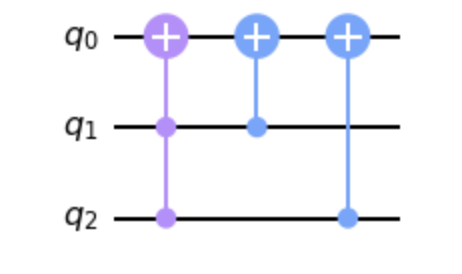
\includegraphics[scale=0.7]{reversibleOr.png}
  \end{minipage}
&
\begin{minipage}[t]{0.43\linewidth}
  \begin{verbatim}
  cx  q[1], q[0];
  x   q[1];
  ccx q[1], q[2], q[0];
  x   q[1];
  \end{verbatim}
  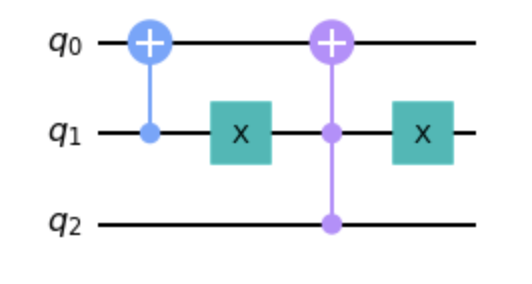
\includegraphics[scale=0.6]{reversibleOr2.png}
  \end{minipage}
\end{tabular}

\medskip

There is a wealth of manual and algorithmic approaches for producing circuits such
as the two above~\cite{maslov:2003:rls:1087512,1201583}. The circuit on the left
was manually produced using a standard synthesis algorithm for reversible
circuits~\cite{10.1145/775832.775915}. The circuit on the right was produced
using an approach that analyzes the recursive structure of the circuit (and
would generalise to computing the disjunction of more than two inputs):

From the specification of the circuit, we expect input \verb|011| to be mapped
to \verb|111|. To gain some intuition, we trace the evaluation of each circuit for
input \verb|011|. In this context, the most significant bit is at index 0. In
the first circuit, the \verb|ccx| gate negates \verb|q[0]| since both \verb|q[1]| and
\verb|q[2]| are true producing \verb|111|; the following \verb|cx| gate produces
\verb|011|; finally the last \verb|cx| produces the result \verb|111|. For the
second circuit, the trace of the execution on the same input value \verb|011| goes through the stages \verb|111|, \verb|101|, \verb|101|, and finally \verb|111|.

Although rather trivial, the examples above illustrate the general idea. A more
interesting example would be the classical core of Shor's algorithm which
requires a circuit implementing $f(r) = a^{r} \mod N$ for fixed $a$ and $N$. The
specification of the circuit is relatively straightforward to calculate. Here it
is for $a=11$ and $N=15$:
\[\begin{array}{rcll}
g(r,h) &=& \left\{ \begin{array}{ll}
                     (r,h+1) & \mbox{when~$r$~even~and~$h$~even} \\
                     (r,h-1) & \mbox{when~$r$~even~and~$h$~odd} \\
                     (r,11-h) & \mbox{when~$r$~odd~and~$4 > h \geq 0$~or~$12 > h \geq 8$} \\
                     (r,19-h) & \mbox{when~$r$~odd~and~$8 > h \geq 4$~or~$16 > h \geq 12$}
                                \end{array}\right.
\end{array}\]

\noindent However, as explained in standard accounts of the algorithm (e.g., the
Qiskit implementation), producing an efficient modular exponentiation circuit
from this specification is not straightforward and is actually the bottleneck in
Shor’s algorithm. Typical derivations of the circuit start from elementary
gates, build a circuit for reversible disjunction (like the two circuits above),
reversible conjunction, a circuit for a half-adder, a circuit for computing the
carry, progressing to a circuit for modular addition, which is used to build a
circuit for modular multiplication, and then finally a circuit for modular
exponentiation taking care at each step to avoid the exponential blowup (e.g.,
by implementing exponentiation by squaring instead of repeated
multiplication)~\cite{shorefficient}.

% To make the connection to reversible computing explicit, we use the Agda
% formalisation of our technical result to extract various computational
% procedures to synthesise, normalise, optimise, and verify reversible
% circuits. In this introduction,

% From the definition of $\underline{\vee}$ it is evident that setting $h=0$, we can compute the desired disjunction by observing the first component of the result. The $\mathit{reversibleOr}$ function has the following truth table (in binary on the left and in a more convenient decimal notation on the right):

% \begin{center}\begin{tabular}{|ccc|ccc|@{\qquad\qquad}|c|c|}
% 0 & 0 & 0 &     0 & 0 & 0     & 0 & 0 \\
% 0 & 0 & 1 &     1 & 0 & 1     & 1 & 5 \\
% 0 & 1 & 0 &     1 & 1 & 0    & 2 & 6 \\
% 0 & 1 & 1 &     1 & 1 & 1    & 3 & 7 \\
% 1 & 0 & 0 &     1 & 0 & 0    & 4 & 4 \\
% 1 & 0 & 1 &     0 & 0 & 1    & 5 & 1 \\
% 1 & 1 & 0 &     0 & 1 & 0    & 6 & 2 \\
% 1 & 1 & 1 &     0 & 1 & 1    & 7 & 3
% \end{tabular}\end{center}

% \noindent where it is evident that it is a bijective function, i.e., reversible.

% As a simple example for that middle stage, we synthesise a reversible circuit
% implementing boolean disjunction ($\vee$). Following~\citet{Toffoli:1980}, the
% first step is to write a specification for the desired reversible function:

% The above embedding of an irreversible function into a reversible function with
% additional inputs and outputs is completely general and is the starting point
% for specifications of quantum circuits. The challenge is to synthesise a program
% / circuit from this specification. Of course, writing this program in a
% conventional (irreversible) language defeats the purpose. The challenge is to
% construct the desired program / circuit exclusively using reversible primitives,
% e.g.,

% the standard set of universal reversible gates used in frameworks like
% Qiskit which consists of the computational gates \textsf{not} (boolean negation,
% called \verb|x|), \textsf{cnot} (conditional negation of the second input if the
% first is true; called \verb|cx|), and \textsf{toffoli} (conditional negation of
% the third input if both the first two inputs are true; called \verb|ccx|) gates,
% and the ability re-arrange the layout of wires.
